\chapter{Task 1 - Object Spawning}
In this chapter, the scene graph will be discussed and how the objects were displayed on screen. The setup of the game will also be discussed so that subsequent sections will flow more easily.

The following files were downloaded from VLE and used as is without modification:
\begin{itemize}
	\item \textbf{light.js}
	\item \textbf{material.js}
	\item \textbf{model.js}
	\item \textbf{matrix.js}
\end{itemize}

The following scripts were downloaded and modified slightly:

\begin{itemize}
	\item \textbf{textures.js}: Removed previous textures and added new ones (listed below) and put the \textit{convertTextures} function inside it.
	\begin{itemize}
		\item wood: used for the bricks
		\item wood2: used for platform
		\item wood3: used for the walls
		\item iron: used for the balls
		\item gold: used for the powerups
		\item oil: used for the bullets
	\end{itemize}

	\item \textbf{scene.js}: Added a \textit{removeNode} function, which takes a string parameter, traverses the scene graph using a depth-first search and when it finds the node with a child whose name corresponds to the given name, sets that child to null and returns.
\end{itemize}

An important script is \textbf{game.js}. This contains important game parameters and variables which are used throughout the game. It contains parameters about the following (in the order in which they are presented in the code [which contains very useful comments])
\begin{itemize}
	\item Number of lives
	\item Wall positions
	\item Number of bricks (rows and columns - for procedural generation)
	\item Platform parameters
	\item Camera parameters
	\item Ball parameters
	\item Powerup parameters
\end{itemize}

Besides these parameters, \textbf{game.js} also contains the physics objects which are used in the game. An array '\textit{keyDown}' of size 256 is initialised to all \textit{false}. When a key on the keyboard is pressed, the index corresponding to the key turns to true, until it is let go at which point the index turns to false again. This is a way to easily detect whether a key is held down or not. For more specific details on the parameters, the comments describe each parameter and its use.

For events which only happen once when a key is pressed down, the \textit{onKeyDown} method is defined. This method, for example, handles the shooting of bullets. A corresponding method \textit{onKeyUp} is also defined, which releases the ball when spacebar is released after being pressed. These two methods are also the functions where the '\textit{keyDown}' elements are set to true or false accordingly.

The \textbf{modelMaker.js} file contains the given \textit{makeSphere} and \textit{makeQuad} functions. \textit{makeSphere} is used for the balls, powerups, bullets and particles. Alongside these, the functions \textit{makeRectangle} and \textit{makeCuboid} were made, which take the dimensions and positions of said shape and generate the vertices for these shapes. The make cuboid makes 6 quads for the 6 faces and combines them together. This is used for the bricks, platforms and walls.

The file \textbf{objectPool.js} contains a function \textit{ObjectPool} which aids object pooling. A pool is defined by the developer, then the function \textit{getNext} can be used to rotate (iterating where the 'queue' is circular so when it reaches the end, it start from the beginning) trough the objects in the pool. This is done as both an optimisation as well as a simplification step, so that objects do not need to be continuously created and destroyed. These pools are used for the particles, additional balls, bullets and powerups.

Within the \textbf{script.js} file, the rest of the functionality happens. This file contains the \textit{main} function which does the following (in order):
\begin{enumerate}
	\item Defines helper variables for matrices and vectors
	\item Sets up the canvas
	\item Initialises the game variable from \textbf{game.js} and adds its \textit{onKeyUp} and \textit{onKeyDown} methods to the event listeners
	\item Initialise the scene graph
	\item Creates a sphere and cuboid primitive (of unit lengths/radius and position origin)
	\item Sets up geometry for the items (walls, platform, balls, bricks, powerups, bullets and particles)
	\item Creates physics objects for each required item (discussed in the physics section) (Note: while 1 brick can be defined in regards to geometry, then replicated within the scene graph, each single brick would need its own physics item. This is the same for any object for which there are multiple)
	\item Sets up the different lights
	\item Initialise textures from \textbf{textures.js}
	\item Create the separate materials
	\item Assign the materials to the objects
	\item Sets up the scene graph (Discussed below)
	\item Creates the animate function which handles movement (discussed in the physics section)
	\item Calls the animate function
\end{enumerate}

The following is an image of the scene at the start of a game:
\begin{figure}[H]
	\centering
	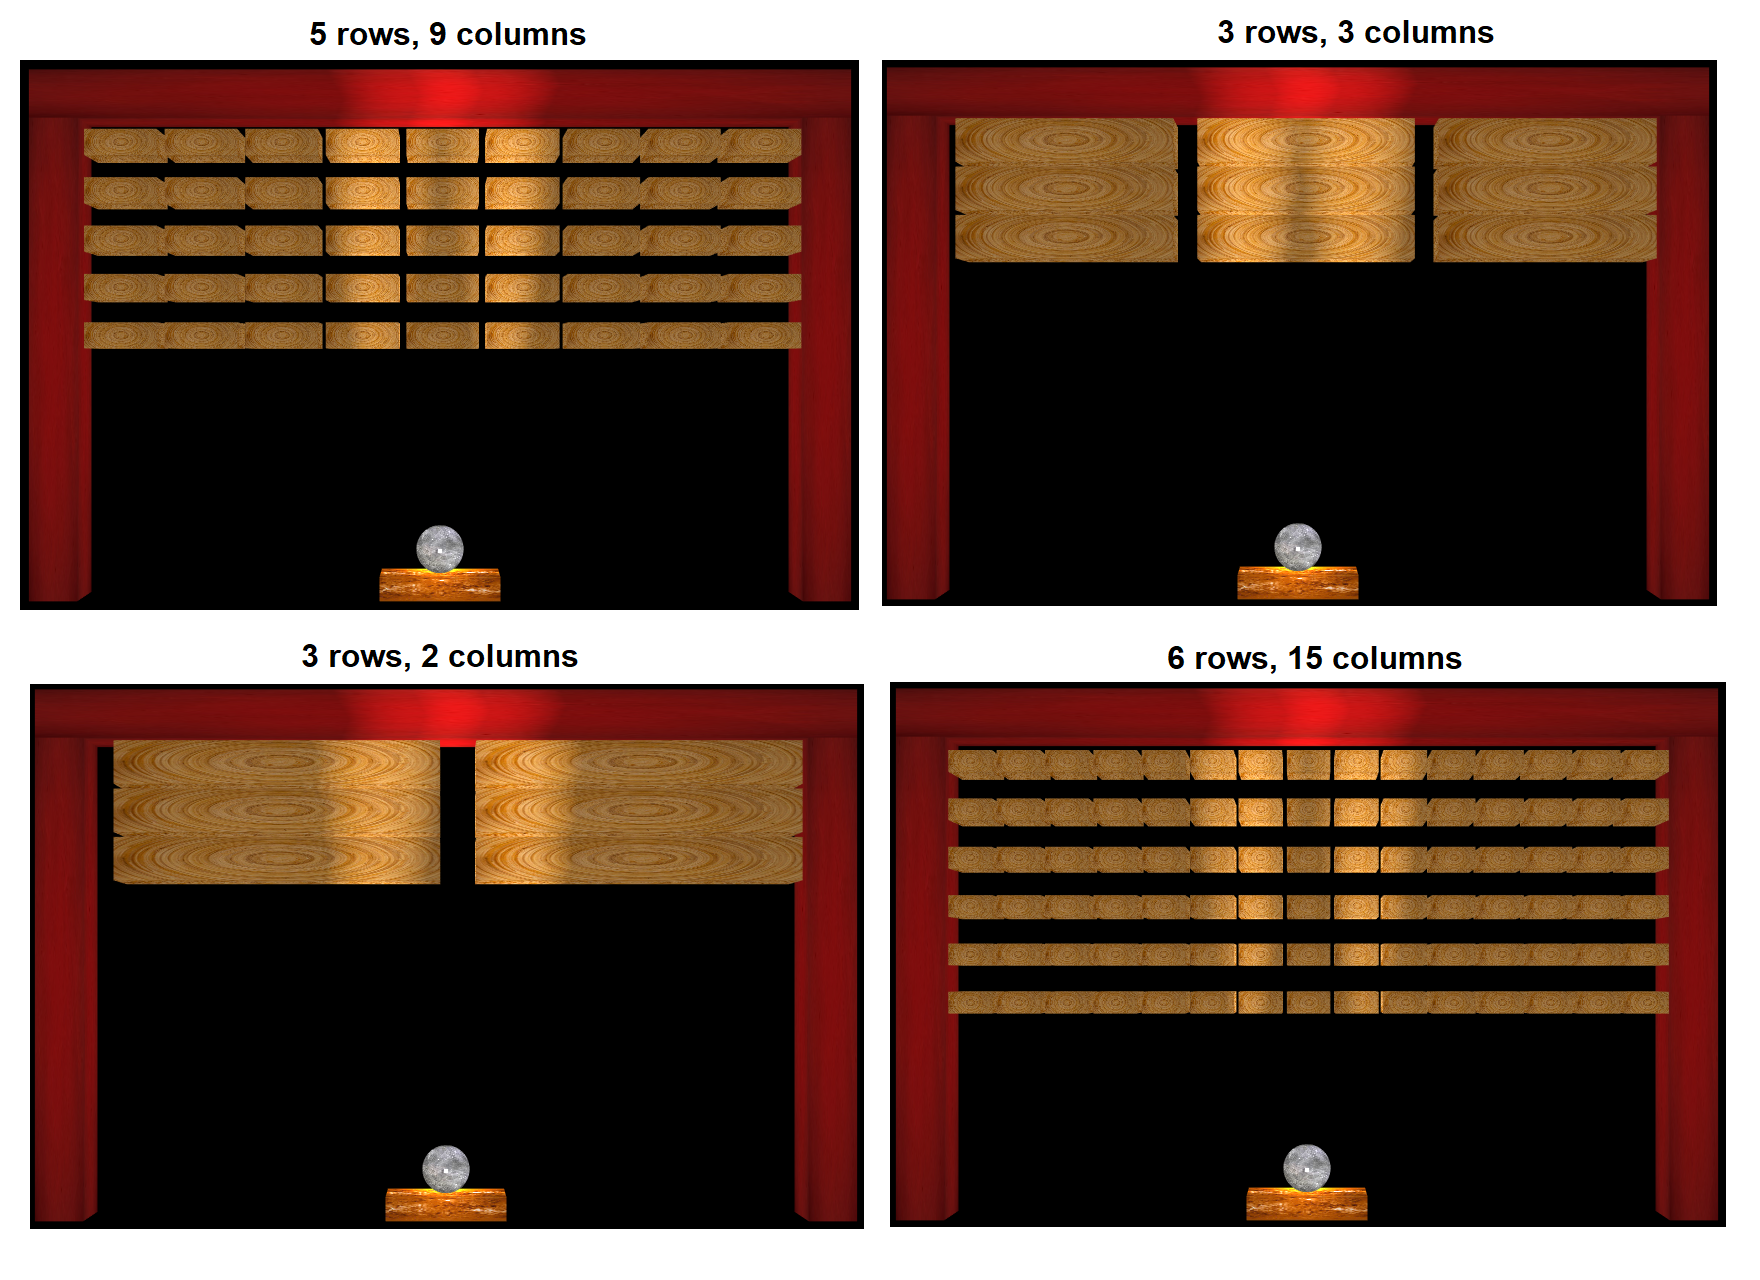
\includegraphics[width=\textwidth]{Images/SceneStart.png}
	\caption{Image at the start of the scene with different number of bricks. Number of rows and columns can be defined from \textbf{game.js}}
\end{figure}

The scene graph used was a simple one. Essentially it first goes trough all the lights, so that each object is affected by each light source, then everything else is initialised. The movements are instead handled by the physics system.
\begin{figure}[H]
	\centering
	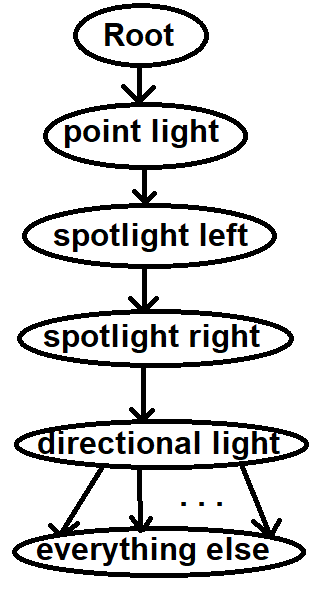
\includegraphics[width=0.3\textwidth]{Images/SceneGraph.png}
	\caption{Graphical representation of the scene graph}
\end{figure}

The appropriate materials are applied to the objects, with the proper materials to make them diffuse and specular as necessary. The walls, bricks and platform are diffuse, while the balls, powerups and bullets have a specular material.